\section{Hot Malware Family Mining}
\label{sec:hot}

\begin{figure*}[!htb]
\minipage{0.22\textwidth}
  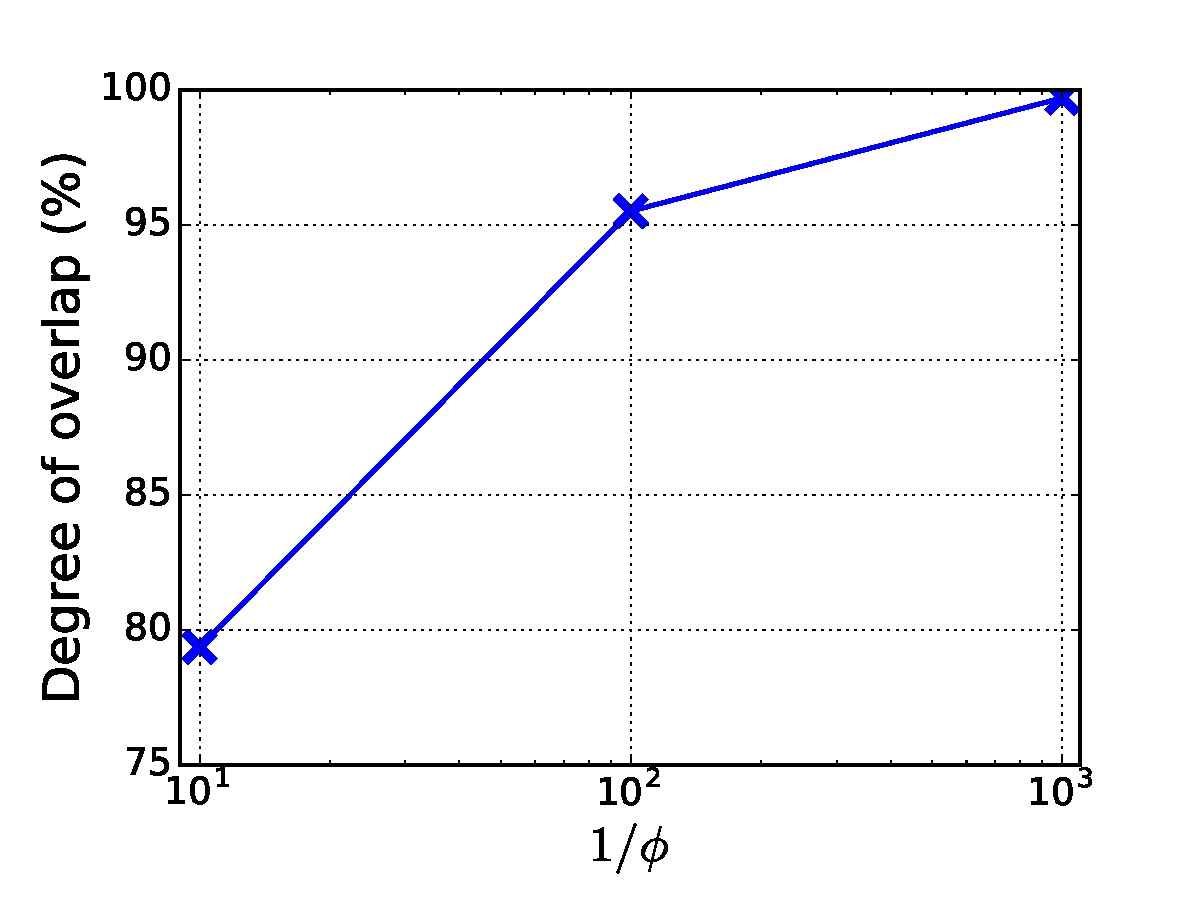
\includegraphics[width=\linewidth]{figure/overlap.pdf}
  \caption{Relation between $\phi$ and degree of overlap.}
  \label{fig:overlap}
\endminipage\hfill
\minipage{0.22\textwidth}
  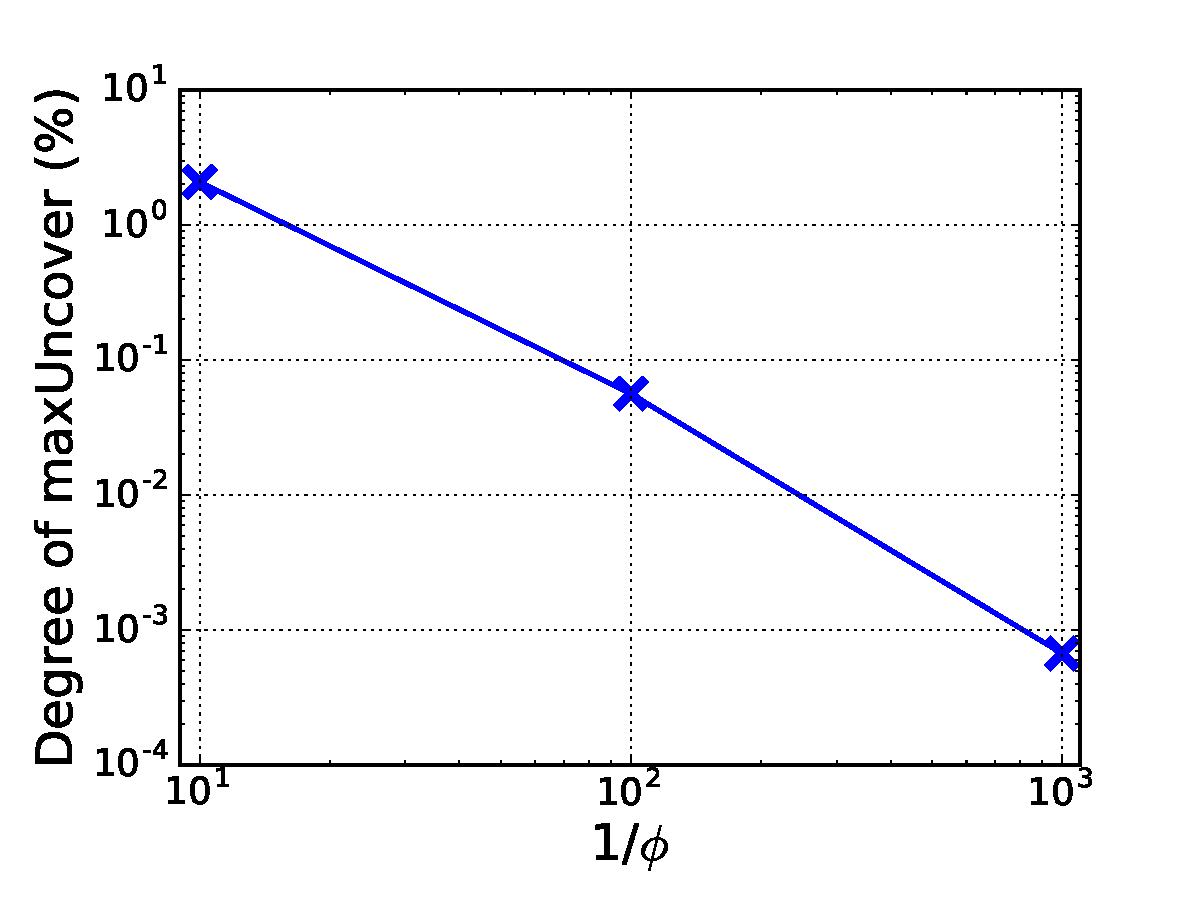
\includegraphics[width=\linewidth]{figure/maxUncover.pdf}
  \caption{Relation between $\phi$ and degree of maxUncover.}
  \label{fig:maxUncover}
\endminipage\hfill
\minipage{0.22\textwidth}%
  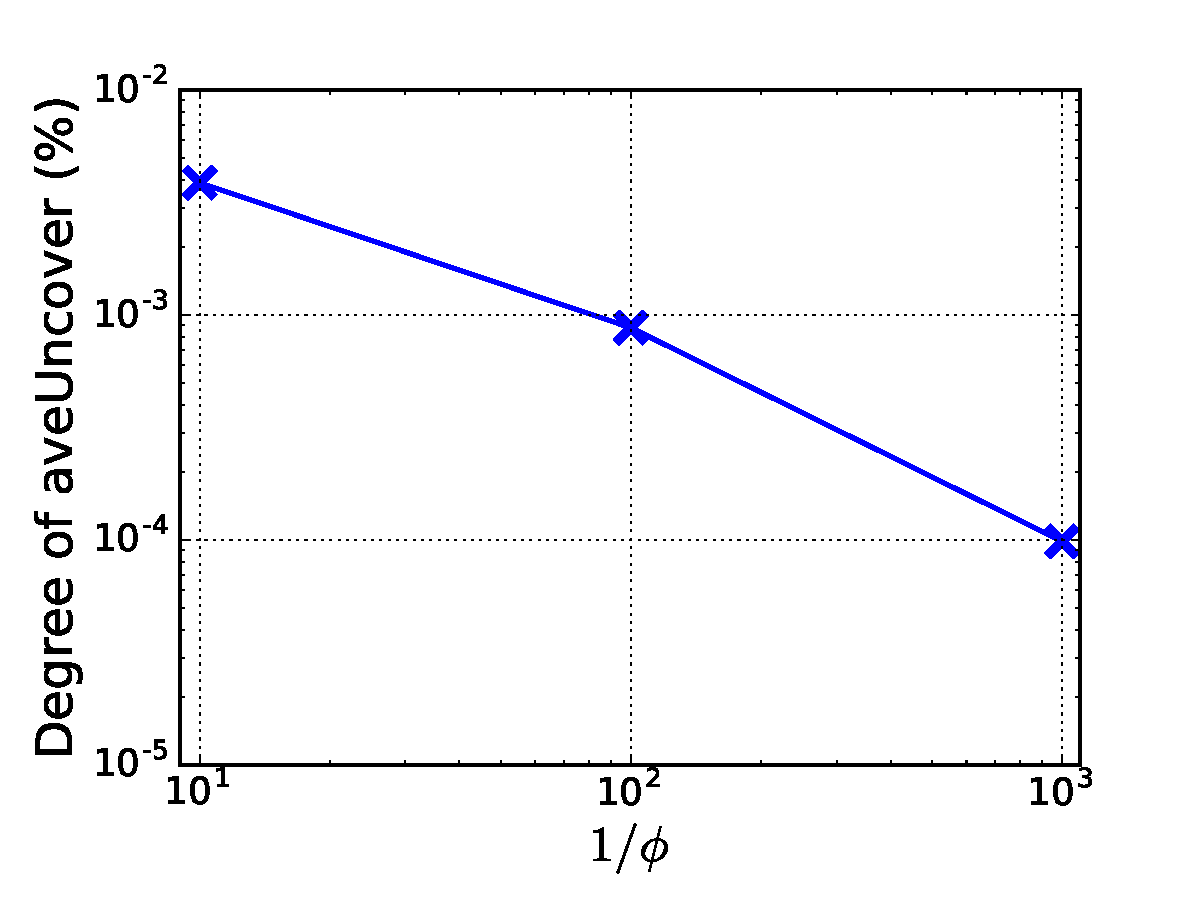
\includegraphics[width=\linewidth]{figure/aveUncover.pdf}
  \caption{Relation between $\phi$ and degree of aveUncover.}
  \label{fig:aveUncover}
\endminipage\hfill
\minipage{0.22\textwidth}%
  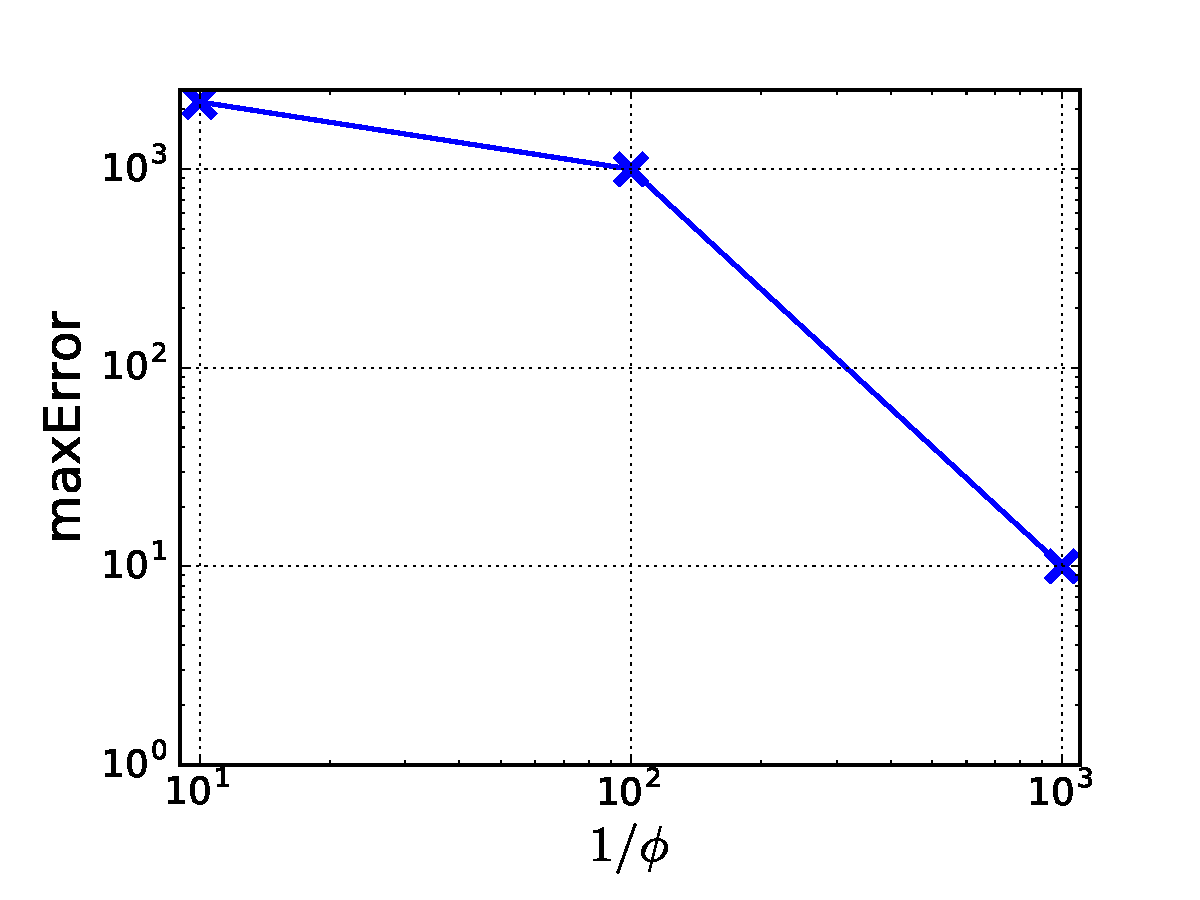
\includegraphics[width=\linewidth]{figure/maxError.pdf}
  \caption{Relation between $\phi$ and maximum error.}
  \label{fig:maxError}

\endminipage
\end{figure*}

\begin{figure}[t!]
\begin{center}
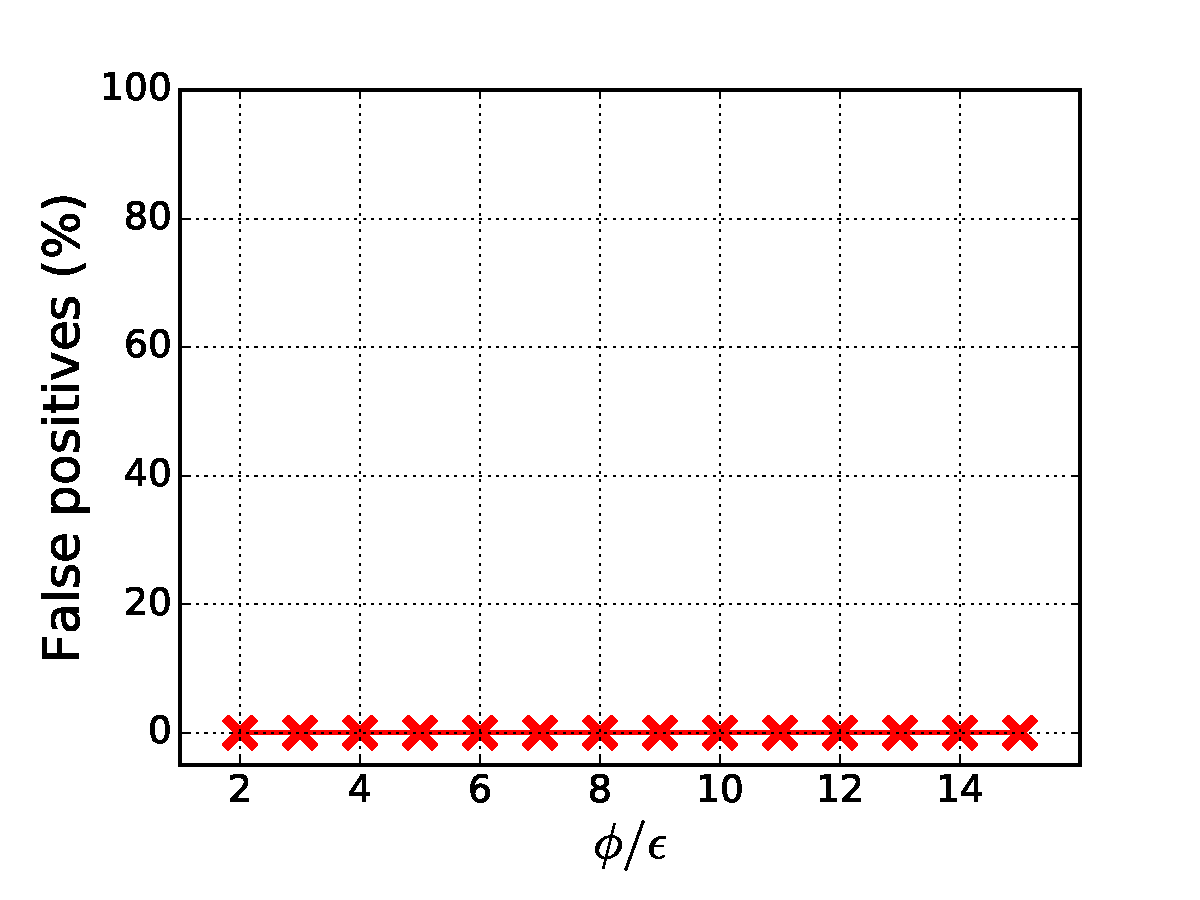
\includegraphics[width=3.0in]{figure/fp}
\caption{FP number.}
\label{fig:new}
\end{center}
\end{figure}

In this section, we view data on VirusTotal as a stream, according to each submission's timestamp, 
and apply a frequent item mining algorithm to identify hot malware family. 

Frequent item mining algorithms take two configuration parameters, $\phi$ and $\epsilon$, where $\phi > \epsilon$. 
The goal of frequent item mining algorithms are to provide nearly-real time analysis on massive data streams by using constant memory. 
Assuming the length of the input stream is N, the output of frequent item mining algorithms 
are all items which appear more than $\lfloor \phi N \rfloor$, 
and no items which appear less than  $\lfloor \epsilon N \rfloor$. 

The frequent item mining algorithm we use is space saving algorithm~\cite{space-saving}, 
which was proposed for streams in Internet advertising, and has already been applied in other areas, 
like mining hot calling contexts in profilers~\cite{hot-calling-context}.
Space saving algorithm tracks $M=1/\epsilon$ pairs of $(f, c)$. 
$f$ is short for malware family, and $c$ is short for counter.  
Pair content represents $(\phi, \epsilon)\mbox{-}HMF$ (Hot Malware Family). 
The M pairs are initialized with the first M encountered malware families and their frequency. 
When a new malware submission comes, 
if the malware family is already under monitored, 
the related counter will be increased by 1. 
And if the malware family is not monitored, 
we will replace the malware family of the pair with lowest counter value with the new malware family, 
and increase its counter value by 1. 
When querying HMF, 
all malware families whose counter values are larger than $\lfloor \phi N \rfloor$ will be returned. 


Following previous works in frequent item mining~\cite{hot-calling-context}, 
we will measure the following metrics by using malware submission date we collect:

Degree of \textit{overlap} is used to measure the percentage of malwares covered in $(\phi, \epsilon)\mbox{-}HMF$,
and it is defined as follows:

$$overlap((\phi, \epsilon)\mbox{-}HMF) = \dfrac{1}{N}\sum_{f \in (\phi, \epsilon)\mbox{-}HMF}w(f)$$

In the above equation, $N$ represents the total number of malware submissions, and 
$w(f)$ represents the real frequency of malware family $f$.  

\textit{maxUncover} (maximum frequency of uncovered malware families) and 
is used 
to measure largest frequency of malware familiy not covered in $(\phi, \epsilon)\mbox{-}HMF$. 
They are defined as follows:
$$maxUncover((\phi, \epsilon)\mbox{-}HMF) = \max_{f \notin (\phi, \epsilon)\mbox{-}HMF}w(f)$$

\textit{aveUncover} (average frequency of uncovered malware families) is defined similarly. 

\textit{False positives} are defined as malware families returned during querying HMF, but whoese
real frequencies are less than $\lfloor \phi N \rfloor$. 

\textit{maxError} is used to measure relative error of counter values, compared with real frequencies.
It is defined as follows:

$$maxError((\phi, \epsilon)\mbox{-}HMF) = \max_{f \in (\phi, \epsilon)\mbox{-}HMF} \dfrac{\left|c(f) - w(f)\right|}{w(f)}$$





